\section{Control y manejo de un quadrotor}
Un cuadricóptero, también conocido como \textit{quadrotor}, es un vehículo aéreo no tripulado que utiliza cuatro rotores para generar sustentación y controlar su movimiento. Este tipo de dron posee seis grados de libertad, ya que puede desplazarse en los ejes \(x\), \(y\) y \(z\), y también puede rotar alrededor de sus tres ejes principales mediante los ángulos de roll \((\phi)\), pitch \((\theta)\) y yaw \((\psi)\). El roll corresponde a la inclinación lateral, el pitch a la inclinación hacia adelante o hacia atrás, y el yaw a la rotación del dron sobre su eje vertical.\cite{kim2020quadrotorSurvey}

\begin{figure}[H]
    \caption{\textbf{Sistema de coordenadas y fuerzas de un cuadricóptero.}}
    \centering
    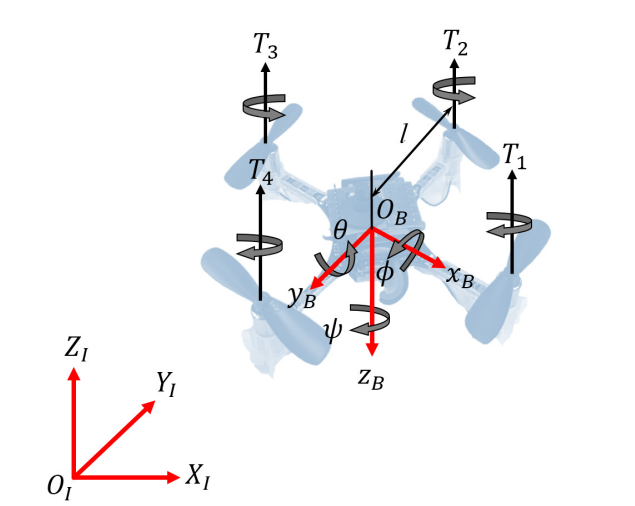
\includegraphics[width=0.55\linewidth]{cuadrupedo_marco_ref.png}
    \caption*{\textit{Nota.} La imagen muestra el sistema de coordenadas inercial y el sistema de coordenadas del cuerpo de un cuadricóptero. Imagen obtenida de \cite{kim2020quadrotorSurvey}.}
    \label{fig:sistema_coordenadas_cuadricoptero}
\end{figure}
\section{Plataforma crazyflie 2.1}
El Crazyflie 2.1 es un mini cuadricóptero versátil y de código abierto desarrollado por la empresa Bitcraze. Esta plataforma tiene un peso aproximado de 29 g y dimensiones de 92×92×29 mm, lo que la hace adecuada para aplicaciones de investigación, educación y pruebas en espacios interiores. La comunicación con el dron se hace por medio de la antena crazyradio 2.0, esta es una antesna de baja latencia.

La arquitectura del Crazyflie 2.1 puede entenderse a partir de dos componentes principales de procesamiento. El primero es el microcontrolador nRF51822, encargado principalmente de la comunicación por radio, Bluetooth de baja energía, lógica de encendido, gestión de batería y detección de placas de expansión. El segundo es el microcontrolador STM32F405, que realiza las tareas principales de control de vuelo, lectura de sensores, telemetría y control de motores.

Una parte importante de esta arquitectura es el \textit{Commander Framework}, encargado de recibir los \textit{setpoints} o referencias deseadas de movimiento. Estos setpoints pueden representar una posición, velocidad u orientación que el dron debe alcanzar. A partir de estas referencias, el sistema de control interno intenta llevar el estado estimado del Crazyflie hacia el estado deseado. \cite{bitcraze_stabilizer_module}

\begin{figure}[H]
    \centering
    \caption{Flujo del módulo estabilizador.}
    \label{fig:flujo_modulo_estabilizador}
    
    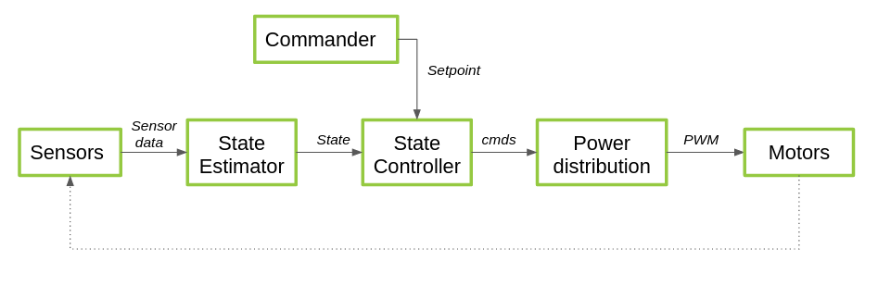
\includegraphics[width=0.75\linewidth]{Commander_framework.png}
    
    \vspace{2mm}
    \begin{flushleft}
        \footnotesize
        \textit{Nota.} La figura muestra el flujo de información desde los sensores hasta los motores dentro del módulo estabilizador del Crazyflie 2.1. Adaptado de Bitcraze \cite{bitcraze_stabilizer_module}.
    \end{flushleft}
\end{figure}
\section{Filtro Kalman y control de Crazyflie 2.1}

El filtro de Kalman es un método matemático utilizado para estimar el estado de un sistema dinámico a partir de información proveniente de un modelo y de mediciones realizadas por sensores. Su utilidad principal es que permite combinar distintas fuentes de información, incluso cuando estas presentan ruido, errores o diferentes frecuencias de actualización. De esta manera, el sistema puede obtener una estimación más confiable que la que se tendría al utilizar únicamente un sensor de forma independiente.\cite{kalman1960}

En el caso del Crazyflie 2.1, el dron cuenta con sensores internos que le permiten estimar su movimiento y estabilidad, como el acelerómetro, el giroscopio y el barómetro. Estos sensores entregan información importante sobre la orientación, aceleración y comportamiento dinámico del dron. Sin embargo, por sí solos no siempre son suficientes para conocer con precisión la posición absoluta del dron dentro de un espacio de trabajo, ya que pueden presentar ruido o acumulación de error durante el vuelo.\cite{schwendener2025desarrollo}

Por esta razón, para lograr un vuelo estable y preciso resulta útil incorporar mediciones externas de posición y orientación. La plataforma Crazyflie permite integrar información proveniente de sistemas del \textit{MoCap}, los cuales permiten conocer la pose del dron dentro del espacio de trabajo. Esta información se introduce al filtro de Kalman extendido, donde se combina con los datos de los sensores internos para mejorar la estimación del estado del dron \cite{bitcraze_state_estimation}.
\begin{figure}[H]
    \centering
    \caption{Entradas y salidas del filtro de Kalman extendido del Crazyflie.}
    \label{fig:ekf_mocap}

    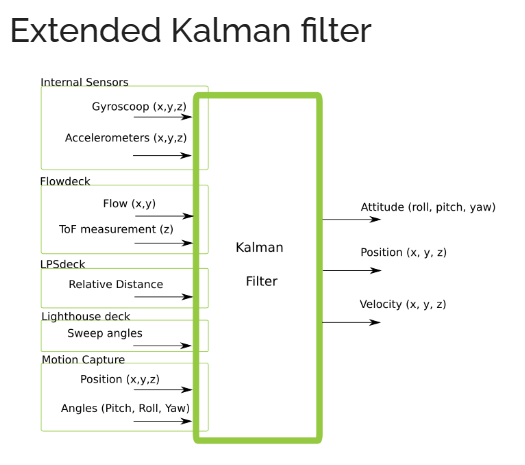
\includegraphics[width=0.78\linewidth]{Extended_Kalman_Filter.png}

    \vspace{2mm}
    \begin{flushleft}
        \footnotesize
        \textit{Nota.} La figura muestra las distintas fuentes de medición que pueden alimentar el filtro de Kalman extendido del Crazyflie. \cite{bitcraze_state_estimation}.
    \end{flushleft}
\end{figure}
\section{Sistemas de captura de movimiento}

Un sistema de captura de movimiento (\textit{Motion Capture}, MoCap) permite registrar la posición y orientación de un objeto dentro de un espacio tridimensional definido. En los sistemas ópticos basados en marcadores, las cámaras registran la luz reflejada o emitida por marcadores colocados sobre el objeto o sujeto de interés. A partir de estas detecciones, el sistema reconstruye la posición tridimensional de los marcadores y permite representar digitalmente su movimiento dentro del volumen de captura .

Existen distintos tipos de marcadores utilizados en sistemas MoCap. Los marcadores pasivos no emiten luz propia, sino que reflejan la luz infrarroja emitida por las cámaras. Por otro lado, los marcadores activos incorporan un emisor de luz, generalmente infrarroja, que permite su detección por parte del sistema. En ambos casos, los marcadores se adhieren al objeto o cuerpo de interés para que el sistema pueda reconstruir su movimiento a partir de sus posiciones en el espacio. \cite{ghorbani2021soma}

Los sistemas ópticos pasivos con marcadores reflectivos y cámaras infrarrojas son ampliamente utilizados debido a que no generan interferencias electromagnéticas y resultan poco intrusivos, ya que únicamente requieren colocar marcadores sobre la superficie del objeto. Sin embargo, presentan limitaciones cuando los marcadores quedan obstruidos de la línea de visión de las cámaras, ya que esto puede provocar pérdida de información o errores en la reconstrucción del movimiento. Además, en sistemas complejos puede ser necesario utilizar una mayor cantidad de cámaras y marcadores, lo cual incrementa el costo y la complejidad de la instalación \cite{schwendener2025desarrollo}.

En el ecosistema Robotat, el sistema MoCap disponible es de tipo pasivo y está conformado por  6 cámaras OptiTrack con un área de trabajo de 400 X 500 X 200 cm. Este sistema permite obtener información de posición absoluta de los objetos dentro del espacio de trabajo con variaciones milimétricas, lo que lo convierte en una herramienta adecuada para aplicaciones de control y seguimiento de trayectorias en interiores \cite{schwendener2025desarrollo}. Para este trabajo, esta característica es especialmente importante, ya que el sistema MoCap puede utilizarse tanto para conocer la posición del Crazyflie 2.1 como para registrar los movimientos del usuario durante la ejecución de gestos.

